\section{Metodologia badań}
W tym rozdziale przedstawiono metodologię przeprowadzonych badań, środowisko testowe oraz wybrane algorytmy do badań środowisk uruchomieniowych.

\subsection{Środowisko testowe}
Do przeprowadzenia testów został wykorzystany system operacyjny Linux Ubuntu 22.04.03, zainstalowany w (ang. \textit{ang. Windows Subsystem for Linux}). Wybór ten dodatkowo jest podyktowany faktem iż do momentu pisania niniejszej pracy, środowisko Bun nie udostępniło oficjalnego wsparcia dla systemu Windows.

Wybór powyższego systemu jest podyktowany faktem, że jest to system, na którym wybrane środowiska są najczęściej uruchamiane. Badanie wykonane w 2015 roku, pokazuje iż większość osób odpowiedzialnych za administrowanie aplikacjami webowymi korzysta z systemu Linux \cite{performance_comparison_linux}. Kolejnym badaniem przeprowadzonym w 2021 roku, pokazało iż sam system jest bardziej wydajny niż Windows Server \cite{web_server_performance}. Badania także pokazało, że większość serwerów internetowych działa na systemie Linux. W związku z tym, wybór systemu Linux jest uzasadniony.

Wymienione środowiska posługują się swoimi implementacjami programów umożliwiających uruchamianie programów opartych o Javascript, staje się to problematyczne w przypadku użycia języka TypeScript. Aby uruchomić skrypty napisane za pomocą tego języka TypeScript należy je stranspilować do języka Javascript. W przypadku NodeJs, powstały odpowiednie paczki tj.: \textit{ts-node} \cite{ts_node}, \textit{tsx} \cite{tsx}. Potrafią one przetworzyć pliki napisane w TypeScript do Javascript. W przypadku Deno oraz Bun, ta funkcjonalność jest wbudowana w środowisko, pozwala to na zrezygnowanie z dodatkowych narzędzi.

Środowiska także inaczej podchodzą do zapisu plików na urządzeniach. We wszystkich środowiskach można zapisać oraz odczytać plik za pomocą metod synchronicznych jak i asynchronicznych. Środowisko Bun udostępnia swoją implementacje zapisy oraz odczytu wykorzystując swoje metody asynchroniczne. Dodatkowym atutem samego środowiska Bun jest możliwość użycia bibliotek, które są odpowiednikiem dla tych dostępnych w NodeJs. W przypadku Deno, zapis oraz odczyt odbywa się za pomocą dekoderów oraz enkoderów, które odczytują tekst w zadanym formacie.

\section{Wybrane narzędzi i algorytmy}
W tym rozdziale znajdują się algorytmy wykorzystane w testach wydajnościowych dla każdego środowiska uruchomieniowego. Wraz z podaniem opisu algorytmu, znajduje się także opis zastosowania algorytmu w praktyce.

\subsection{Algorytmy sortowania}
W testach zostały wykorzystane trzy algorytmy sortowania, które są najczęściej wykorzystywane w praktyce. Sortowanie jako metoda jest używana w wielu zastosowaniach, takich jak sortowanie danych w bazach danych, sortowanie danych w aplikacjach webowych, a także w algorytmach wyszukiwania. W teście sortowania został przeprowadzone testy na losowo wybranych liczbach całkowitych.

Liczby całkowite zostały wylosowane za pomocą generatora liczb całkowitych. Do samej implementacji generatora liczb całkowitych posłużył pakiet \textit{Math}, który jest dostępny w języku JavaScript. Generator został zaimplementowany tak, aby losował liczby w zależności od zadanego rozmiaru tablicy.

Każdy z algorytmów charakteryzuje się inną złożonością obliczeniową, co wpływa na czas sortowania danych. Możemy to zauważyć w pracy \cite{sorting}, gdzie pokazywane są czasy poszczególnych algorytmów sortowania. W tabeli \ref{tab:sorting_complexity} przedstawiono złożoności obliczeniowe dla poszczególnych algorytmów.

\begin{table}[h]
  \centering
  \begin{tabular}{|l|l|l|l|}
  \hline
  \textbf{Algorytm Sortowania} & \textbf{Optymistyczna} & \textbf{Średnia} & \textbf{Pesymistyczna} \\ \hline
    Bubble Sort & $O(n)$ & $O(n^2)$ & $O(n^2)$ \\ 
    \hline
    Quick Sort & $O(n log n)$ & $O(n log n)$ & $O(n^2)$ \\ 
    \hline
    Radix Sort & $O(nk)$ & $O(nk)$ & $O(nk)$ \\
    \hline
  \end{tabular}
  \caption{Złożoność obliczeniowa dla algorytmów sortowania}
  \label{tab:sorting_complexity}
\end{table}

\subsubsection{Sortowanie bąbelkowe (\textit{ang. Bubble Sort})}
Sortowanie bąbelkowe (\textit{ang. Bubble Sort}) to jeden z najprostszych algorytmów sortowania. Algorytm ten działa poprzez porównywanie dwóch sąsiadujących elementów i zamianę ich miejscami, jeśli są w niewłaściwej kolejności. Złożoność obliczeniowa algorytmu w pesymistycznym wypadku wynosi $O(n^2)$.

Działanie algorytmu można określić w kilku krokach:
\begin{enumerate}
  \item Przejdź przez tablicę od początku do końca.
  \item Dla każdego elementu, sprawdź czy sąsiedni element jest mniejszy od obecnego.
  \item Jeśli sąsiedni element jest mniejszy, zamień miejscami obecny element z sąsiednim.
  \item Powtarzaj kroki 1-3, aż tablica zostanie posortowana.
\end{enumerate}

Algorytm ten jest jednym z najwolniejszych algorytmów sortowania, jednakże jest on prosty w implementacji. W przypadku małych zbiorów danych, algorytm ten jest wystarczający, jednakże w przypadku dużych zbiorów danych, algorytm ten może być bardzo wolny. W najlepszym wypadku, gdy tablica jest już posortowana złożoność obliczeniowa wynosi $O(n)$, co oznacza, że algorytm ten jest szybki w przypadku posortowanych danych.

\subsubsection{Sortowanie szybkie (\textit{ang. Quick Sort})}
Quick Sort to jeden z najpopularniejszych i najwydajniejszych algorytmów sortowania ogólnego przeznaczenia. Został opracowany przez Tony'ego Hoare'a w 1960 roku. Algorytm działa na zasadzie "dziel i zwyciężaj" (\textit{ang. divide and conquer}), co oznacza, że dzieli w przypadku testów tablicę liczb całkowitych na mniejsze tablice, które są następnie rozwiązywane rekurencyjnie.

Działanie algorytmu można określić w kilku krokach:
\begin{enumerate}
  \item Wybierz element z tablicy, który nazywamy elementem osiowym (\textit{ang. pivot}). Sam algorytm wybiera element pierwszy z tablicy jako \textit{pivot}.
  \item Podziel tablicę na dwie części: jedną z elementami mniejszymi od elementu osiowego, a drugą z elementami większymi od elementu osiowego.
  \item Rekurencyjnie posortuj obie części.
  \item Połącz obie części w jedną posortowaną tablicę.
  \item Zwróć posortowaną tablicę.
\end{enumerate}

Zaletą algorytmu jest to, że w porównaniu do algorytmu sortowanie pozycyjnego, nie wymaga on dodatkowego alokowania pamięci na tablice tymczasowe, pracuje on na oryginalnej tablicy. Można zauważyć z tabeli \ref{tab:sorting_complexity}, że algorytm w najgorszym wypadku ma złożoność obliczeniową $O(n^2)$, co oznacza, że w przypadku dużej ilości danych, algorytm ten może być wolniejszy od innych algorytmów sortowania.

\subsubsection{Sortowanie pozycyjne (\textit{ang. Radix Sort})}
Radix Sort to wydajny algorytm sortowania stosowany do porządkowania liczb całkowitych lub innych danych, które można reprezentować jako krotki o stałej długości. Algorytm działa na zasadzie sortowania pozycyjnego, czyli sortowania cyfr od najmniej znaczącej do najbardziej znaczącej (lub odwrotnie, w zależności od implementacji). Dzięki temu możliwe jest osiągnięcie bardzo dobrych wyników czasowych w przypadku dużych zbiorów danych. Złożoność obliczeniowa w przypadku sortowania pozycyjnego wynosi $O(nk)$, gdzie $n$ to liczba elementów do posortowania, a $k$ to liczba cyfr w największym elemencie zbioru.

Działanie algorytmu można określić w kilku krokach:
\begin{enumerate}
  \item Zainicjowanie samego algorytmu podając mu tablicę liczb całkowitych do posortowania.
  \item Dla każdej liczby znalezienie cyfry najmniej znaczącej i umieszczenie jej w odpowiednim kubełku.
  \item Powtarzaj krok 2 dla każdej cyfry, aż do osiągnięcia najbardziej znaczącej cyfry.
\end{enumerate}

Dzięki swojej złożoności obliczeniowej sortowanie pozycyjne jest szybkie, jednakże posiada wadę w postaci konieczności alokowania dodatkowej pamięci, aby przechowywać tymczasowe wyniki sortowania. Jednakże w przypadku danych, które nie są danymi liczbowymi należy przekształcić je na dane liczbowe, co może wpłynąć na czas sortowania. W przypadku danych, które są liczbami, algorytm ten jest jednym z najszybszych algorytmów sortowania \cite{sorting}. W testach dla ujednolicenia danych, zostały zastosowane liczby całkowite.

\subsection{Algorytmy Kodowania}
W testach został wykorzystany jeden algorytm kodowania, który jest najczęściej wykorzystywany do przesyłania danych. Wybrany algorytm kodowania jest Base64. Wykorzystywany jest on do kodowania obrazów, danych wykorzystywanych w formularzach, a także do przedstawiania plików pdf na stronach.

Algorytm możemy podzielić na trzy etapy. Pierwszym etapem jest podział danych na segmenty składające się z 24 bit. Następnie każdy z segmentów jest dzielony na cztery grupy po 6 bitów. Każda grupa zostaje mapowana na z jeden ze znaków:
\begin{itemize}
  \item Litery A-Z (26 znaków)
  \item Litery a-z (26 znaków)
  \item Cyfry 0-9 (10 znaków)
  \item Znaki "+" i "/"
\end{itemize}
W przypadku gdy grupy nie są wielokrotnością liczby 24, wtedy grupy zostają uzupełnione zerami, co przekształca się w znak \textit{=} w celu wskazania liczby dodanych bitów. Na rys \ref{fig:base64_mapping_table} przedstawiono tablicę mapowań dla algorytmu szyfrowania Base64.

\begin{figure}[H]
  \centering
  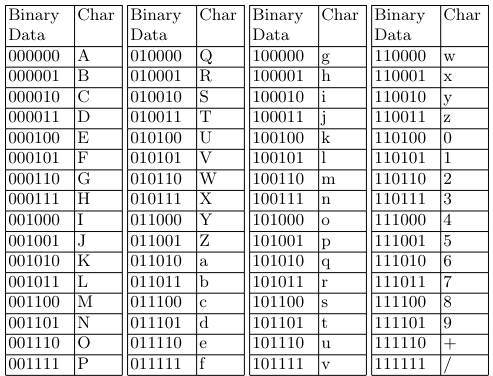
\includegraphics[width=0.6\textwidth]{Figures/base64_mapping_table.png}
  \caption{Tablica mapowań dla algorytmu szyfrowania Base64}
  \label{fig:base64_mapping_table}
\end{figure}

Algorytm ten jest przydatny do małych obrazów, jednakże w przypadku dużych obrazów, algorytm ten nie jest zalecany. Wynika to z faktu iż sam algorytm powoduje zwiększenia rozmiaru danych. Dodatkowo wykazano, że w zależności od języka programowania oraz implementacji algorytmu, czas kodowania oraz dekodowania może się różnić \cite{cryptoeprint:2022/361}.

Test został zaimplementowany z wykorzystaniem obiektu \textit{Buffer} odpowiedzialnego za kodowanie oraz dekodowanie wartości zakodowanych wiadomości. Oryginalny test wykonany przez Kostya \cite{base64_benchmark}, został zmodyfikowany, aby dodać informacje o czasie wykonywania oraz użyciu pamięci przez dane środowisko. Test ten został przeprowadzony w celu sprawdzenia jak szybko dane środowisko jest w stanie zakodować oraz odkodować dane.

\subsection{Bazy danych}
W testach została wykorzystana plikowa baza relacyjna Sqlite3. Wybór ten podyktowany jest faktem iż baza ta ma wsparcie dla wszystkich środowisk uruchomieniowych. Celem testu było zmierzenie czasu odpowiedzi bazy danych na zapytania SQL. 

W celu dodania do bazy danych przykładowych danych została wykorzystany pakiet \textit{faker-js}. Pakiet ten pozwala na generowanie obiektów z danymi losowymi. W celu przetestowania możliwości bazy danych, została opracowany model, który odzwierciedla użytkownika. Model ten składa się z pól takich jak: imię, nazwisko, płeć, opis, typ wykonywanej pracy, tytuł oraz zakres pracy. Test pozwala na specyfikowania ilości rekordów, które mają zostać dodane do bazy danych.

W przypadku NodeJs, wymagane jest aby zainstalować dodatkowy pakiet odpowiedzialny za komunikację z bazą danych. W odróżnieniu do pozostałych środowisk, które posiadają wbudowane wsparcie dla Sqlite3. Przez dodanie nowych pakietów, powiększa się rozmiar aplikacji, wpływa to na rozmiar oraz czas uruchamiania się aplikacji.

\subsection{Narzędzia pomiarowe}
W celu zmierzenia czasów wykonania poszczególnych testów, zostały wykorzystane narzędzia dostępne w języku JavaScript. Do mierzenia czasu wykonania danego testu została wykorzystana moduł \textit{performance}. Moduł ten pozwala na zapisanie czasu w postaci milisekund, co pozwala na dokładne określenie czasu wykonania danego testu. Metoda wykorzystuje obiekt \textit{DOMHighResTimeStamp}, który pozwala na określenie czasu w milisekundach z dokładnością do 5 mikrosekund.

W celu zmierzenia 